\section{Test}
Vi blev bedt om at lave en \textbf{J-unit} test af vores felttypers \texttt{landOnField} metoder. Disse vil være beskrevet i dette afsnit.
\subsection{Test af Refuge}
Sammen med opgaven fik vi et bilag, der beskrev hvordan testen af \texttt{Refuge} skulle laves.


Til formålet oprettes en testklasse \texttt{RefugeTest}. I denne klasse tog vi indholdet fra bilagene, og modificerede det lidt. For at få koden til at passe til vores program ændrede vi nogle småting. Da vi har benyttet os af \textbf{BCE} notationen til vores pakker, måtte vi importere vores \texttt{Player} til at oprette objekter igennem \texttt{intity} pakken. Samtidig har vi kun en metode til både at trække penge og give penge på en spillers konto. Derfor har vi slettet \texttt{Neg200} funktionerne i  alle tests. Derfor bestemmer konsekvensen af feltypen i stedet, om der skal trækkes eller indsættes penge. Kørslen af testen ses i figur \vref{fig:testrefuge}.
\begin{figure}[!ht]
\centering
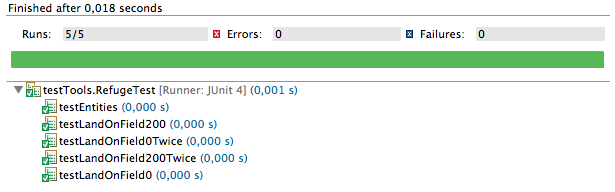
\includegraphics[width=0.8\textwidth]{RefugeTest.jpg}
\caption[<Text for the list of figures>]{Resultatet af testkørsel Refuge}
\label{fig:testrefuge} 
\end{figure}
\subsection{Test af Laborcamp}
\texttt{LaborCampTest} er stort set magen til. Her har vi bare trukket beløbet fra på \texttt{expected}, da vores felttype nu giver en negativ konsekvens for spilleren. Samtidig har vi omdøbt pointerne til \textit{Field}, så de hedder noget med \texttt{labor}. Kørslen af testen ses i figur \vref{fig:labor}.
\begin{figure}[!ht]
\centering
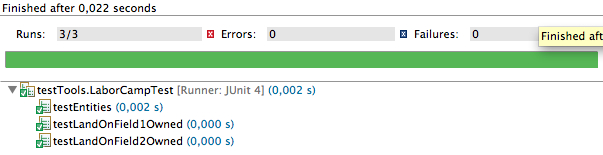
\includegraphics[width=0.8\textwidth]{LaborTest.jpg}
\caption[<Text for the list of figures>]{Resultatet af testkørsel LaborCamp}
\label{fig:labor} 
\end{figure}
\subsection{Test af Tax}
Den første testklasse til \texttt{TaxTest}, er præcis magen til \texttt{LaborCampTest}. Bortset fra vi har skiftet navnene, så de passer til denne testklasse.  Kørslen af testen ses i figur \vref{fig:testtax}.
\begin{figure}[!ht]
\centering
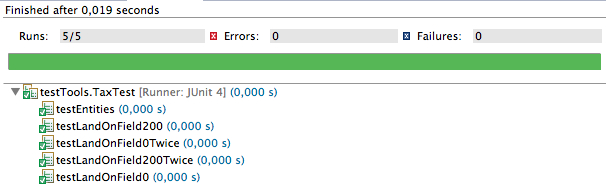
\includegraphics[width=0.8\textwidth]{TaxTest.jpg}
\caption[<Text for the list of figures>]{Resultatet af testkørsel Tax}
\label{fig:testtax} 
\end{figure}
\subsection{Test af Fleet}
Testen af \texttt{Fleet} krævede en lille smule mere arbejde. Her var vi nødt til at oprette vores \texttt{Gameboard}, for at kune sætte en ejer på vores \texttt{Fleet}. Dette gjorde vi på samme måde, som vi satte vores \texttt{player} nemlig med \texttt{this.owner = new Player(1000, "Andersine");} Vi opretter også vores \texttt{Fleet} felter \texttt{this.gameBoard.setField(new Fleet("Fleet1", 0, gameBoard), 18);}. Vi fortæller nu, hvilke felt vores \texttt{owner} har, og hvilket felt vores \texttt{player} står på, og så er det ellers stort set samme procedure som de andre tests. Kørslen af testen ses i figur \vref{fig:fleet}.
\begin{figure}[!ht]
\centering
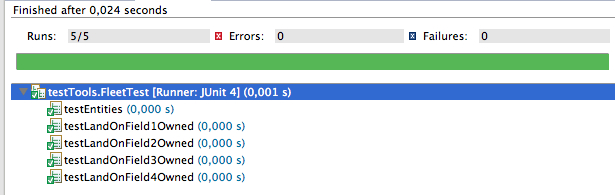
\includegraphics[width=0.8\textwidth]{FleetTest.jpg}
\caption[<Text for the list of figures>]{Resultatet af testkørsel Fleet}
\label{fig:fleet} 
\end{figure}
\subsection{Test af Territory}
Denne testklasse er bygget op på stort set samme måde som \texttt{Fleet} med en \texttt{owner} og en \texttt{player}. Det eneste specielle er at vi bliver nødt til at kalde \texttt{((Ownable)ter200).setOwner(owner);} for at kunne sætte ejeren. Kørslen af testen ses i figur \vref{fig:testter}.
\begin{figure}[!ht]
\centering
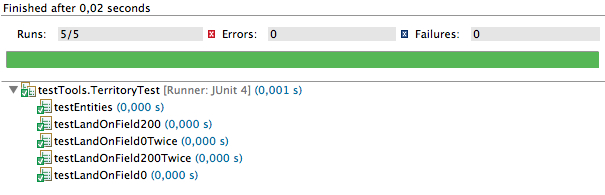
\includegraphics[width=0.8\textwidth]{TerTest.jpg}
\caption[<Text for the list of figures>]{Resultatet af testkørsel Territory}
\label{fig:testter} 
\end{figure}
\subsection{Test og fejlfinding generelt}
Vi har genbrugt vores "snydeterning" fra sidste projekt, som vi har brugt til lettere at lande på bestemte felter, når vi skulle teste en bestemt felttype.
Ellers har vi benyttet os de \textbf{White Box} tests, der var lavet en \textbf{Junit} skabelon til.

Ud over det har vi lavet en enkelt \textbf{User Test}, da al vores kode var færdig. Lige som sidst skabte det forvirring, at spillet skulle startes i Eclipse, og beskederne kom både i konsol og via \textbf{GUI}.